\newif\ifglobal

%%%%%%%%%%%%%%%%%%%%%%%
%%% Compile to view %%%
%%%%%%%%%%%%%%%%%%%%%%%

%%%%%%%%%%%%%%%%%%%%%%%%%%%%%%%%%%%%%%%%%%%%%%%%%%%
%%% Readme:                                     %%%
%%% https://www.overleaf.com/read/bwdjvfjksvjy/ %%%
%%%%%%%%%%%%%%%%%%%%%%%%%%%%%%%%%%%%%%%%%%%%%%%%%%%

% >>> M?: marks a module setting number or important notice

% >>> M4: Set {./relative-path} to external files for this module <<<
\def \modulefiles {./31-SENSOR}
% To add an external file, use:
% (Replace '---' with actual filename)
% '\input{\modulefiles/tables/---.tex}' for tables
% '\includegraphics{\modulefiles/figures/---}' for figures
% '\subfile{\modulefiles/---}' for register files


% >>> M1: This module is in global project? <<<
% 'YES' - uncomment; 'NO' - comment out
\globaltrue

\ifglobal
    \documentclass[main\_\_CN.tex]{subfiles}

\else
    % Font "FandolSong-Regular" used by ctex does not have GSUB table.
    % It causes warnings that do not affect compilation and can be ignored.
    \PassOptionsToPackage{quiet}{fontspec}

    \documentclass[openany, 10pt]{book}

    % >>> M2: In ./00-shared/preamble-trm-module, also find
    %         settings for visibility of todo notes, watermark <<<
    \usepackage{preamble-trm-module}

    % Enable Chinese typesetting
    \usepackage{ctex}

    % >>> M3: Temporary labels in Chinese
    %         you can add your own labels there <<<
    \myexternaldocument{./00-shared/temp-labels-cn}

\fi %\ifglobal


\setcounter{secnumdepth}{4}


% >>> M5: If this module needs any updates in
% './00-shared/preamble-trm-module.sty'
% (include additional package, etc.), contact your module PM
% or create the file './00-shared/changelog.tex' make the
% necessary updates yourself and document them in this file <<<

% Make text left-aligned and allow latex to break pages naturally, comment out for full justification
\raggedright
\raggedbottom


\begin{document}


% Sets language into which pre-defined bits of text are translated
\selectlanguage{chinese}
\setchineseformatting


% Do not delete this block
\ifglobal
% Add the following front matter if
% this module is outside of global project
\else
    \InputIfFileExists{readme}{}{}
    \listoftodos
    {\let\clearpage\relax \listofdonetodos}
    \tableofcontents
    %\listoftables
    %\listoffigures
\fi


%%%%%%%%%%%%%%%%%%%%%%%%%
%%% TRM Module Begins %%%
%%%%%%%%%%%%%%%%%%%%%%%%%

\hypertarget{sensor}{}
\chapter{片上传感器与模拟信号处理}
\label{mod:sensor}

\section{概述}

ESP32 集成\hyperref[ssec:touch sensor]{电容式触摸传感器}，最高支持 10 路输入。

ESP32 的模拟信号处理主要由 2 个\hyperref[ssec:saradc]{逐次逼近模拟数字转换器} (Successive Approximation ADC, SAR ADC) 完成。系统专门内置了 5 个 ADC 专用控制器，可在转换模拟输入信号时支持高性能与低功耗 2 种模式，处理器的开销最低。

此外，ESP32 还可使用 2 个\hyperref[ssec:dac]{独立数字模拟转换器(DAC)}和 1 个\hyperref[ssec:cosine gen]{余弦波形发生器}生成模拟信号。

\section{电容式触摸传感器}\label{ssec:touch sensor}

\subsection{简介}

触摸传感器系统主要由 3 个部分组成，从外到内依次为平面保护层、电极与基片，见图 \ref{figure:touch sensor}。 当用户触碰保护层时，传感器系统的电容量会发生改变，继而生成 1 个可以反映本次触碰是否触发的二进制信号。

\begin{figure}[!ht]
    \centering
    \fbox{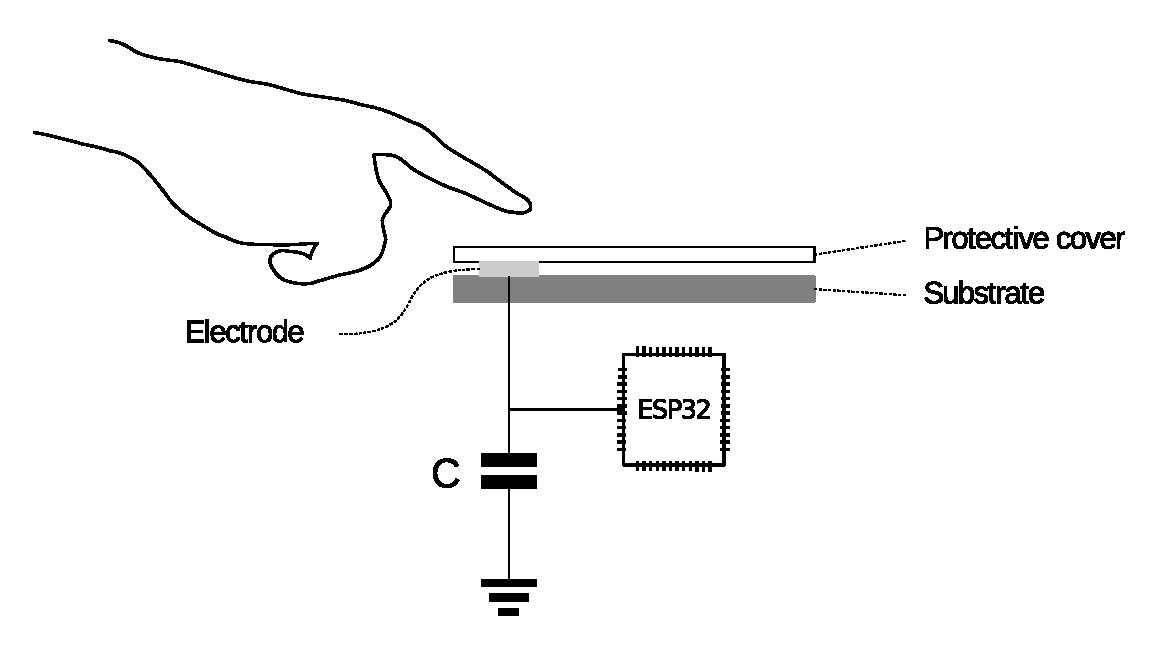
\includegraphics[width=0.6\textwidth]{./31-SENSOR/figures/touchsensor2.eps}}
    \caption{触摸传感器}
    \label{figure:touch sensor}
\end{figure}

\subsection{主要特性}\label{sec:on_chip_sensor_features}

\begin{itemize}
    \item 最多支持 10 路电容触摸管脚/通用输入输出接口(General Purpose Input and Output, GPIO)
    \item 触摸管脚可以组合使用，可覆盖更大触感区域或更多触感点
    \item 触摸管脚的传感由有限状态机(FSM)硬件控制，由软件或专用硬件计时器发起
    \item 触摸管脚是否受到触碰的信息可由以下方式获得：
    \begin{itemize}
        \item 由软件直接检查触摸传感器的寄存器
        \item 由触摸监测模块发起的中断信号判断
        \item 由触摸监测模块上的CPU是否从Deep-sleep中唤醒判断
    \end{itemize}
    \item 支持以下场景下的低功耗工作：
    \begin{itemize}
        \item CPU 处于 Deep-sleep 节能模式，将在受到触碰后逐步唤醒
        \item 触摸监测由超低功耗协处理器(ULP coprocessor)管理 \\
        ULP 用户程序可通过写入与检查特定寄存器，判断是否达到触碰阈值
    \end{itemize}
\end{itemize}

\begin{tiplisting}
ESP32 触摸传感器目前尚无法通过射频抗扰度测试系统 (CS) 认证，应用场景有所限制。
\end{tiplisting}

\subsection{可用通用输入输出接口}

全部 10 个可用通用输入输出接口的信息，请见表 \ref{table:touch pads}。

\begin{longtable}[c]{|p{7.5cm}|p{7.5cm}| }
    \caption{ESP32 电容式触摸传感器的管脚}
    \label{table:touch pads}
    \\\hline
    \rowcolor{lightgray}
    触摸传感信号名 & 管脚\\
    \hline
    \endfirsthead
    \hline
    \rowcolor{lightgray}
    触摸传感信号名 & 管脚\\
    \hline
    \endhead
    \endfoot
    \endlastfoot
    T0  &  GPIO4 \\\hline
    T1  &  GPIO0 \\\hline
    T2  &  GPIO2 \\\hline
    T3  &  MTDO  \\\hline
    T4  &  MTCK  \\\hline
    T5  &  MTDI  \\\hline
    T6  &  MTMS  \\\hline
    T7  &  GPIO27 \\\hline
    T8  &  32K\_XN \\\hline
    T9  &  32K\_XP \\\hline
\end{longtable}

\subsection{功能描述}
\label{figure:touch sensor func desc}

触摸传感器的内部结构请见图 \ref{figure:touch sensor structure}，工作流程请见图 \ref{figure:touch sensor operating flow}。

\begin{figure}[!ht]
    \centering
    \fbox{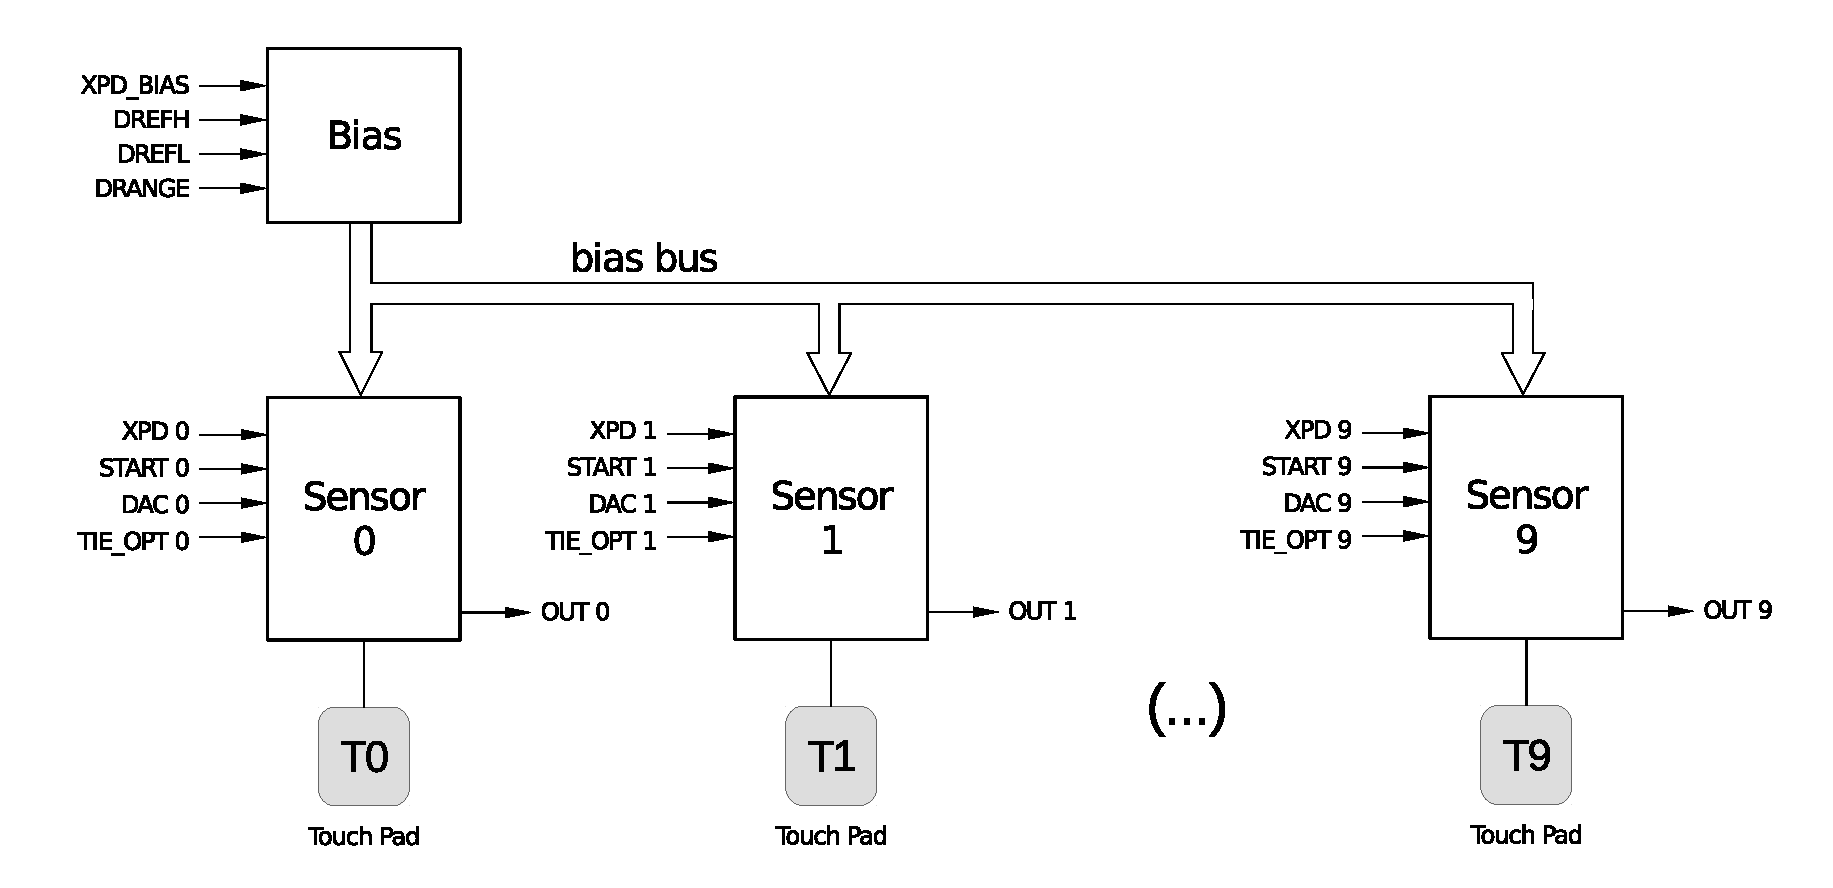
\includegraphics[width=0.7\textwidth]{./31-SENSOR/figures/Touch_Sensor.eps}}
    \caption{触摸传感器的内部结构}
    \label{figure:touch sensor structure}
\end{figure}

触摸管脚的电容会进行周期性充放电。"触摸管脚的内部电压"代表充/放电电压在参考高值 (drefH) 与参考低值 (drefL) 之间的变化。在每次变化中，触摸传感器将生成一个输出脉冲 (OUT)。由于触摸管脚受到触碰（高电容）与未受到触碰（低电容）时的电压变化速率不同，我们可以通过统计同一时间间隔内出现的输出脉冲数量，判断触摸管脚是否受到触碰。可以通过 \hyperref[regdesc:RTCIOTOUCHPADnREG]{TIE\_OPT} 设置开始充/放电的初始电压电平。

\begin{figure}[!ht]
    \centering
    \fbox{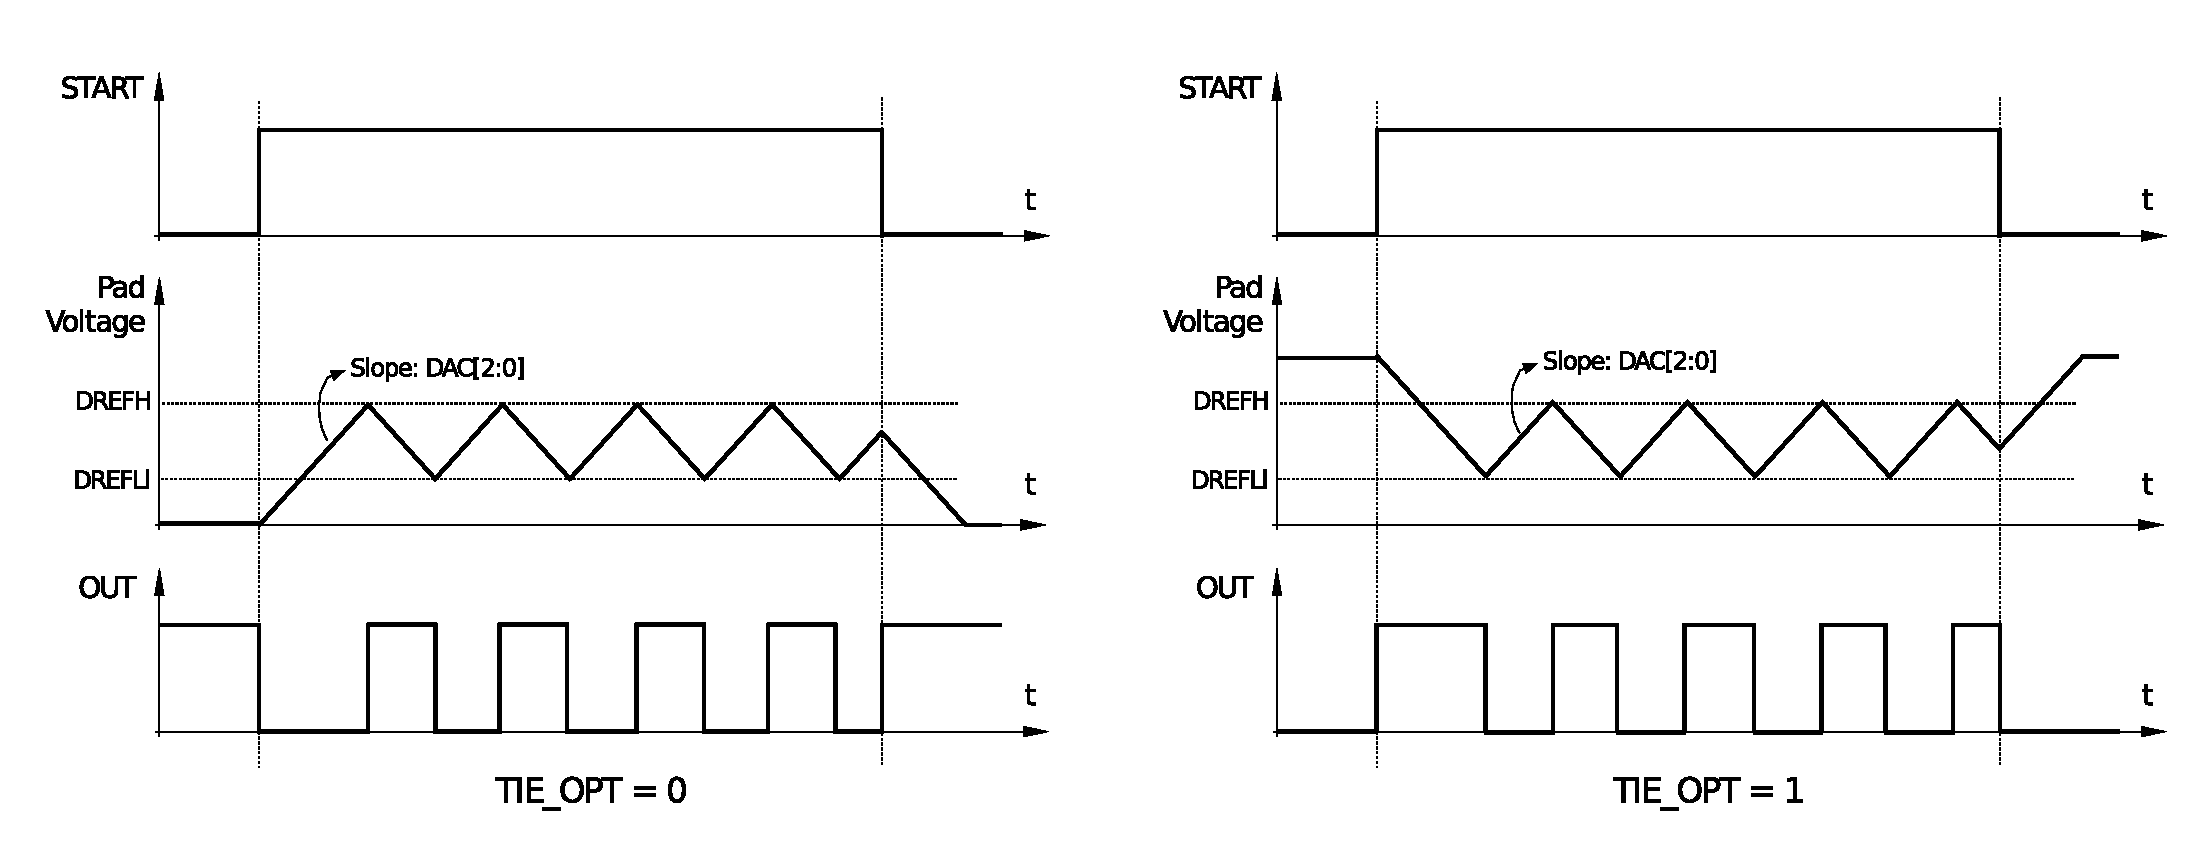
\includegraphics[width=0.9\textwidth]{./31-SENSOR/figures/Touch_Sensor2.eps}}
    \caption{触摸传感器的工作流程}
    \label{figure:touch sensor operating flow}
\end{figure}

\subsection{触发传感器的状态机}

有限状态机 (Finite-State Machine, FSM) 将执行 \ref{figure:touch sensor func desc} 章节描述的序列检测。软件可通过专用寄存器操作 FSM。FSM 的内部结构可见图 \ref{figure:touch fsm}。

FSM 的功能包括：
\begin{itemize}
    \item 接收软件或计时器发出的开始信号
    \begin{itemize}
        \item 当 \hyperref[regdesc:SENSSARTOUCHCTRL2REG]{SENS\_SAR\_TOUCH\_START\_FORCE} = 1 时， 可通过设置 \hyperref[regdesc:SENSSARTOUCHCTRL2REG]{SENS\_SAR\_TOUCH\_START\_EN} 发起一次性检测；
        \item 当 \hyperref[regdesc:SENSSARTOUCHCTRL2REG]{SENS\_SAR\_TOUCH\_START\_FORCE} = 0 时，可利用计时器实现周期性检测。
    \end{itemize}
    触摸传感器在睡眠模式下也能工作。更多信息，请见功耗管理章节。可通过寄存器\\ \hyperref[regdesc:SENSSARTOUCHCTRL2REG]{SENS\_SAR\_TOUCH\_SLEEP\_CYCLES} 设定检测周期。传感器由 RTC\_FAST\_CLK 控制，常见时钟频率为 8 MHz。更多信息，请见\hyperref[mod:resclk]{复位和时钟}章节。
    \item 根据可调节时序，生成 XPD\_TOUCH\_BIAS / TOUCH\_XPD / TOUCH\_START\\
    在选择使能触摸管脚时，TOUCH\_XPD / TOUCH\_START 中的内容将被 10 位寄存器\\ \hyperref[regdesc:SENSSARTOUCHENABLEREG]{SENS\_SAR\_TOUCH\_PAD\_WORKEN} 遮掩。
    \item 计数 TOUCH0\_OUT \verb+~+ TOUCH9\_OUT 上的脉冲数量\\
    计数结果可见 \hyperref[regdesc:SENSSARTOUCHOUT1REG]{SENS\_SAR\_TOUCH\_MEAS\_OUT\textcolor{red}{\it{n}}}。全部 10 个触摸管脚可支持同时工作。
    \item 生成唤醒中断\\
    如果一个管脚的脉冲计数结果低于阈值，则 FSM 视该管脚被“触碰”。10 位寄存器 \hyperref[regdesc:SENSSARTOUCHENABLEREG]{SENS\_TOUCH\_PAD\_OUTEN1} \& \hyperref[regdesc:SENSSARTOUCHENABLEREG]{SENS\_TOUCH\_PAD\_OUTEN2} 可以将所有管脚定义为 2 组，即 SET1 \& SET2。默认状态下，如果 SET1 中的任意管脚被“触碰”，即可生成唤醒中断，也可以配置为 SET1 和 SET2 中均有管脚被“触碰”时有效。
\end{itemize}


\begin{figure}[!ht]
    \centering
    \fbox{
\includegraphics[width=0.9\textwidth]{./31-SENSOR/figures/touch_fsm.eps}}
    \caption{FSM 的内部结构}
    \label{figure:touch fsm}
\end{figure}


\section{SAR ADC}\label{ssec:saradc}

\subsection{简介}

ESP32 内置了 2 个 12 位的 SAR ADC，由 5 个专用转换器控制器管理，可测量来自 18 个管脚的模拟信号。

\begin{figure}[H]
    \centering
    \fbox{
\includegraphics[width=0.7\textwidth]{./31-SENSOR/figures/saradc.eps}}
    \caption{SAR ADC 的概况}
    \label{figure:sar adc overview}
\end{figure}

SAR ADC 使用的 5 个控制器均为专用控制器，其中 2 个支持高性能多通道扫描、2 个经过优化可支持 Deep-sleep 模式下的低功耗运行，另外 1 个专门用于 PWDET / PKDET （功率检测和峰值监测）。SAR ADC 的基本概况见图 \ref{figure:sar adc overview}。

\begin{tiplisting}
PWDET/PKDET 控制器仅供 Wi-Fi 内部使用。如果 Wi-Fi 正在使用 SAR ADC2，则用户无法使用 SAR ADC2 测量管脚的模拟信号。Wi-Fi 释放 SAR ADC2 之后，用户可正常使用 SAR ADC2。
\end{tiplisting} 

\subsection{主要特性}

\begin{itemize}
    \item 采用 2 个 SAR ADC，可支持同时采样与转换
    \item 采用 5 个专用 ADC 控制器，可支持不同应用场景（比如，高性能、低功耗，或功率检测和峰值检测）
    \item 支持 18 个模拟输入管脚
    \item 可配置12 位、11 位、10 位、9 位多种分辨率
    \item 支持 DMA（1 个控制器支持）
    \item 支持多通道扫描模式（2个控制器支持）
    \item 支持 Deep-sleep 模式运行（1 个控制器支持）
    \item 支持 ULP 协处理器控制（2 个控制器支持）
\end{itemize}

\subsection{功能概况}

SAR ADC 的主要元件与连接情况见图 \ref{figure:sar adc functional overview}。

\begin{figure}[H]
    \centering
    \fbox{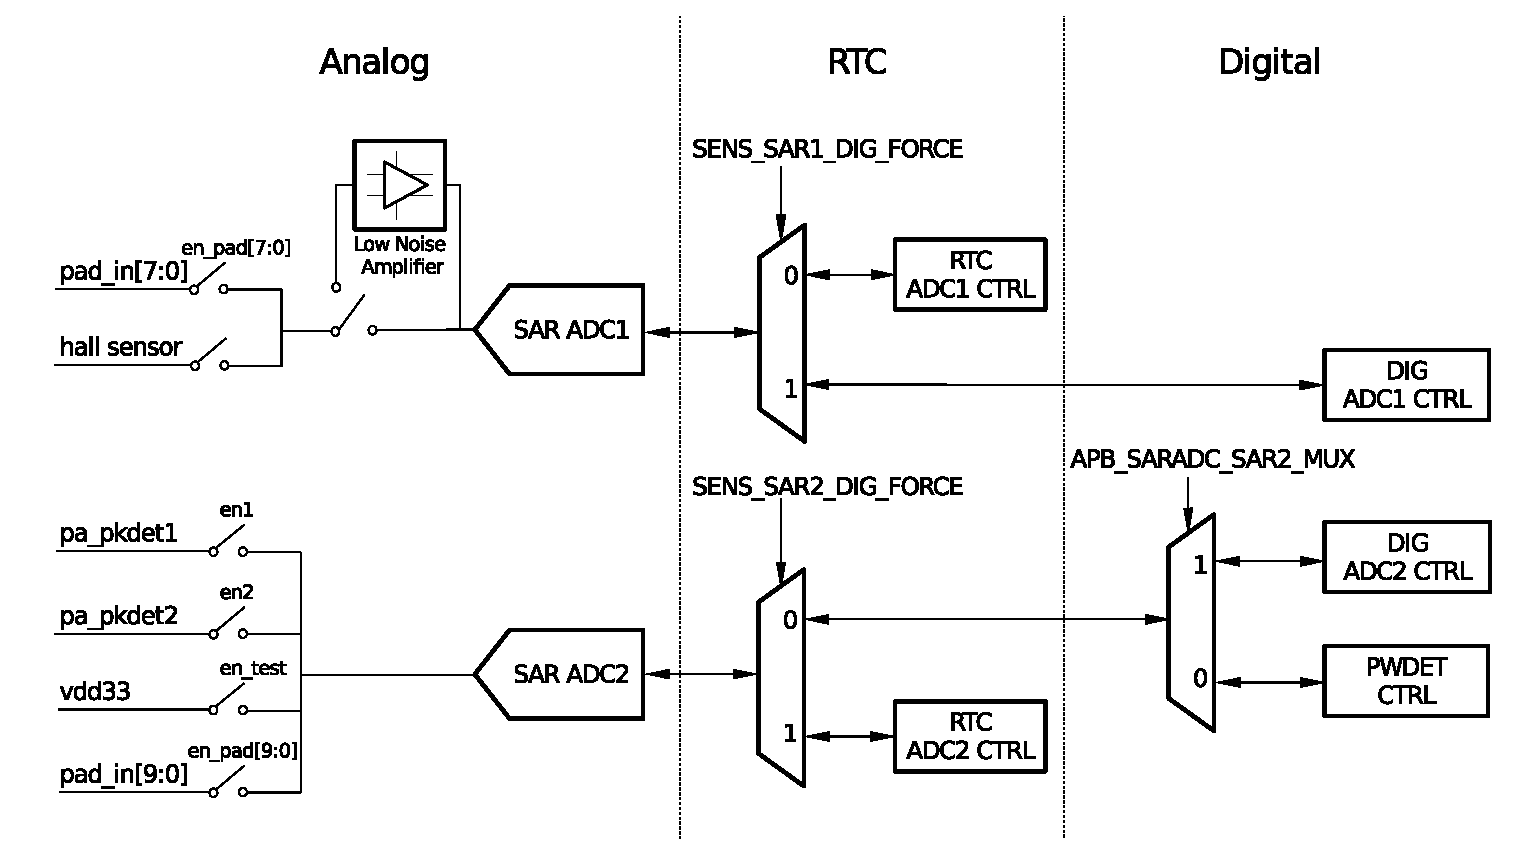
\includegraphics[width=0.9\textwidth]{./31-SENSOR/figures/saradc_mux.eps}}
    \caption{SAR ADC 的功能概况}
    \label{figure:sar adc functional overview}
\end{figure}



表 \ref{table:adc inputs} 列出了 SAR ADC 的信号输入与对应接入的 ADC 信道。

\begin{longtable}{|p{5cm}|p{5cm}|p{2cm}| }
    \caption{SAR ADC 的信号输入}
    \label{table:adc inputs}
    \\\hline
    \rowcolor{lightgray}
    信号名称 &  ADC 信道 \# & ADC 选择 \\\hline
    \endfirsthead
    \hline
    \rowcolor{lightgray}
    信号名称 &  ADC 信道 \# & ADC 选择 \\\hline
    \endhead
    \hline
    \endfoot
    VDET\_2      &  7  & \multirow{8}{*}{SAR ADC1} \\ \cline{1-2}
    VDET\_1      &  6  & \\ \cline{1-2}
    32K\_XN      &  5  & \\ \cline{1-2}
    32K\_XP     &  4  & \\ \cline{1-2}
    SENSOR\_VN    &  3  & \\ \cline{1-2}
    SENSOR\_CAPN   & 2  & \\ \cline{1-2}
    SENSOR\_CAPP   &  1  & \\ \cline{1-2}
    SENSOR\_VP    &  0  & \\ \hline
    GPIO26       &  9  & \multirow{10}{*}{SAR ADC2} \\ \cline{1-2}
    GPIO25      &  8  & \\ \cline{1-2}
    GPIO27      &  7  & \\ \cline{1-2}
    MTMS         &  6  & \\ \cline{1-2}
    MTDI          &  5  & \\ \cline{1-2}
    MTCK          &  4  & \\ \cline{1-2}
    MTDO          &  3  & \\ \cline{1-2}
    GPIO2        &  2  & \\ \cline{1-2}
    GPIO0        &  1  & \\ \cline{1-2}
    GPIO4       &  0  & \\ \cline{1-2}
\end{longtable}
\vspace{-1em}
\begin{tiplisting}
\begin{itemize}
\vspace{-2em}
\item SAR ADC2 的检测管脚中，包括 GPIO0、GPIO2 和 GPIO15 为芯片 Strapping 管脚，用户使用时需特别注意。
\end{itemize}
\end{tiplisting}

ESP32 内置了 5 个专用 ADC 控制器：RTC ADC1 CTRL、RTC ADC2 CTRL、DIG ADC1 CTRL、DIG ADC2 CTRL，及 PWDET CTRL。各控制器的场景支持情况见表 \ref{table:sar adc controllers}。

\begin{longtable}[c]{|p{2.3cm}|p{2.3cm}|p{2.3cm}|p{2.3cm}|p{2.3cm}|p{2.3cm}|}
    \caption{ESP32 的 SAR ADC 控制器}
    \label{table:sar adc controllers}
    \\\hline
    \rowcolor{lightgray}
    & RTC ADC1 & RTC ADC2 & DIG ADC1 & DIG ADC2 & PWDET \\
        \hline
        \endfirsthead
        \hline
        \rowcolor{lightgray}
    & RTC ADC1 & RTC ADC2 & DIG ADC1 & DIG ADC2 & PWDET \\
        \hline
        \endhead
        \endfoot
    DAC                 & Y & - & - & - & - \\\hline
    Deep-sleep          & Y & Y & - & - & - \\\hline
    ULP 协处理器        & Y & Y & - & - & - \\\hline
    PWDET/PKDET         & - & - & - & - & Y \\\hline
    DMA                 & - & - & Y & - & - \\\hline
\end{longtable}


\subsection{RTC SAR ADC 控制器}
\label{sssec:rtcadc}

RTC 电源域中的 SAR ADC 控制器（RTC ADC1 CTRL 和 RTC ADC2 CTRL）可在低频状态下提供最小功耗 ADC 测量。

各控制器的具体功能概况见图 \ref{figure:sar adc ctrl}。对于每个控制器来说，转换是由寄存器  \hyperref[regdesc:SENSSARMEASSTART1REG]{SENS\_SAR\_MEAS\textcolor{red}{\it{n}}\_START\_SAR} 触发，测量结果可见寄存器 \hyperref[regdesc:SENSSARMEASSTART1REG]{SENS\_SAR\_MEAS\textcolor{red}{\it{n}}\_DATA\_SAR}。

\begin{figure}[!ht]
    \centering
    \fbox{
\includegraphics[width=0.8\textwidth]{./31-SENSOR/figures/saradc_rtc_ctrl.eps}}
    \caption{RTC SAR ADC 的功能概况}
    \label{figure:sar adc ctrl}
\end{figure}

ULP 协处理器与控制器之间的关系非常紧密，已经内置了指令来使用 ADC。很多情况下，控制器均需要与 ULP 协处理器协同工作，比如：
\begin{itemize}
    \item 可在 Deep-sleep 模式下对通道进行周期性检测。Deep-sleep 模式下，ULP 协处理器是唯一的触发器。
    \item 可按一定顺序对通道进行连续性扫描。尽管控制器无法支持连续性扫描或 DMA，但 ULP 协处理器可协助实现这部分功能。
\end{itemize}

\subsection{DIG SAR ADC 控制器}
与 RTC SAR ADC 控制器相比，DIG SAR ADC 控制器的性能和吞吐均实现了一定优化，具备以下特点：
\begin{itemize}
    \item 高性能。时钟更快，因此采样速率实现了大幅提升。
    \item 支持多通道扫描模式。每个 SAR ADC 的测量规则可见样式表。扫描模式可配置为单通道模式、双通道模式或交替模式。
    \item 扫描可由软件或 I2S 总线发起。
    \item 支持 DMA。扫描完成即发生中断。
\end{itemize}

\begin{tiplisting}
由于无法通过直接访问发起一次性 SAR ADC 转换，因此我们将在本章节中采用“开始扫描”的说法，代表我们将利用 DIG SAR ADC 控制器扫描一系列通道。
\end{tiplisting}

图 \ref{figure:dig adc overview} 展示了 DIG SAR ADC 控制器的原理图。


\begin{figure}[H]
    \centering
    
\includegraphics[width=0.9\textwidth]{./31-SENSOR/figures/saradc_dma}
    \caption{DIG SAR ADC 控制器的概况}
    \label{figure:dig adc overview}
\end{figure}

样式表可以描述 DIG SAR ADC 控制器需要遵守的各项测量规则，每个表项拥有 16 个项，可存储通道选择、分辨率和衰减信息等内容。当扫描开始时，控制器将逐条读取样式表中的测量规则。对于每个控制器而言，每个扫描序列最多拥有 16 条不同规则。

样式表寄存器的长度为 8 位，共包括 3 个字段，分别存储了通道、分辨率和衰减信息的内容，具体见表 \ref{table:pattern table register}。

\begin{table}[H]
    \caption{样式表寄存器的字段信息}
    \label{table:pattern table register}
    \centering
    \begin{tabular}[c]{|p{5cm}|p{5cm}|p{5cm}|}
        \hline
        \rowcolor{lightgray}
        \multicolumn{3}{|c|}{样式表寄存器[7:0]} \\
        \hline
        ch\_sel[3:0] & bit\_width[1:0] & atten[1:0] \\
        \hline
        扫描通道 & 分辨率 & 衰减 \\
        \hline
    \end{tabular}
\end{table}

扫描模式可配置为：单通道模式、双通道模式或交替模式。

\begin{itemize}
    \item 单通道模式：仅 SAR ADC1 或 SAR ADC2 的通道将被扫描。
    \item 双通道模式：SAR ADC1 和 SAR ADC2 的通道同将被扫描。
    \item 交替模式：SAR ADC1 和 SAR ADC2 的通道将被交替扫描。
\end{itemize}

ESP32 最高支持 12 位的 SAR ADC 分辨率，最终向 DMA 传递的 16 位数据包括 ADC 转换结果，及一些因扫描模式不同而有所差别的相关信息，具体为：

\begin{itemize}
    \item 单通道模式：仅增加 4 位通道选择信息。
    \item 双通道模式或交替模式：增加 4 位通道选择信息，及 1 位 SAR ADC 选择信息。
\end{itemize}

每种扫描模式均有其对应的数据格式，即\uppercase\expandafter{\romannumeral1}型和 \uppercase\expandafter{\romannumeral2} 型。有关这两种数据格式的具体描述，请见表 \ref{table:type i dma data format} 和表 \ref{table:type ii dma data format}。

\begin{table}[H]
    \caption{\uppercase\expandafter{\romannumeral1}型 DMA 数据格式}
    \label{table:type i dma data format}
    \centering
    \begin{tabular}[c]{|p{7.5cm}|p{7.5cm}|}
        \hline
        \rowcolor{lightgray}
        \multicolumn{2}{|c|}{\textbf{\uppercase\expandafter{\romannumeral1}型} DMA数据格式[15:0]} \\
        \hline
        ch\_sel[3:0] & data[11:0] \\
        \hline
        通道 & SAR ADC 信息 \\
        \hline
    \end{tabular}
\end{table}

\begin{table}[H]
    \caption{\uppercase\expandafter{\romannumeral2} 型 DMA 数据格式}
    \label{table:type ii dma data format}
    \centering
    \begin{tabular}[c]{|p{4.85cm}|p{4.85cm}|p{4.85cm}|}
        \hline
        \rowcolor{lightgray}
        \multicolumn{3}{|c|}{\textbf{\uppercase\expandafter{\romannumeral2} 型} DMA 数据格式[15:0]} \\
        \hline
        sar\_sel & ch\_sel[3:0] & SAR ADC data[10:0] \\
        \hline
        {SAR ADC\textcolor{red}{\it{n}}} & 通道 & SAR ADC 信息 \\
        \hline
    \end{tabular}
\end{table}

\uppercase\expandafter{\romannumeral1}型数据格式的 SAR ADC 分辨率最高可支持 12 位，\uppercase\expandafter{\romannumeral2} 型数据格式的 SAR ADC 分辨率最高可支持 11 位。

DIG SAR ADC 控制器允许通过 I2S 总线实现直接内存访问。I2S 总线的 WS 信号可用作测量触发信号。可通过 DATA  信号获得测量结果是否完成的信息。可通过软件配置 \hyperref[regdesc:APBSARADCCTRLREG]{APB\_SARADC\_DATA\_TO\_I2S}，将 ADC 连接至 I2S 总线。

\section{数字模拟转换器}
\label{ssec:dac}

\subsection{简介}

数字模拟转换器 (DAC) 带有 2 个 8 位通道，可将数字值转换为最高 2 路模拟输出信号，包括集成电阻串和缓冲区。这种双通道 DAC 支持将电源当做输入电压参考，且支持双通道的独立/同时转换。

\subsection{主要特性}

DAC的主要特性包括：
\begin{itemize}
    \item 2 个 8 位 DAC 通道
    \item 支持双通道的独立/同时转换
    \item 可从 VDD3P3\_RTC 引脚获得电压参考
    \item 含有余弦波型发生器
    \item 支持 DMA 功能
    \item 可通过软件或 SAR ADC FSM 开始转换。更多信息，请见 \hyperref[ssec:saradc]{SAR ADC} 章节。
    \item 可由 ULP 协处理器通过控制寄存器来实现完全控制。请见 ULP 协处理器章节。
\end{itemize}

单通道 DAC 的功能概况请见图 \ref{figure:dac mux}。具体介绍，请见本章节下方内容。

\begin{figure}[!ht]
    \centering
    \fbox{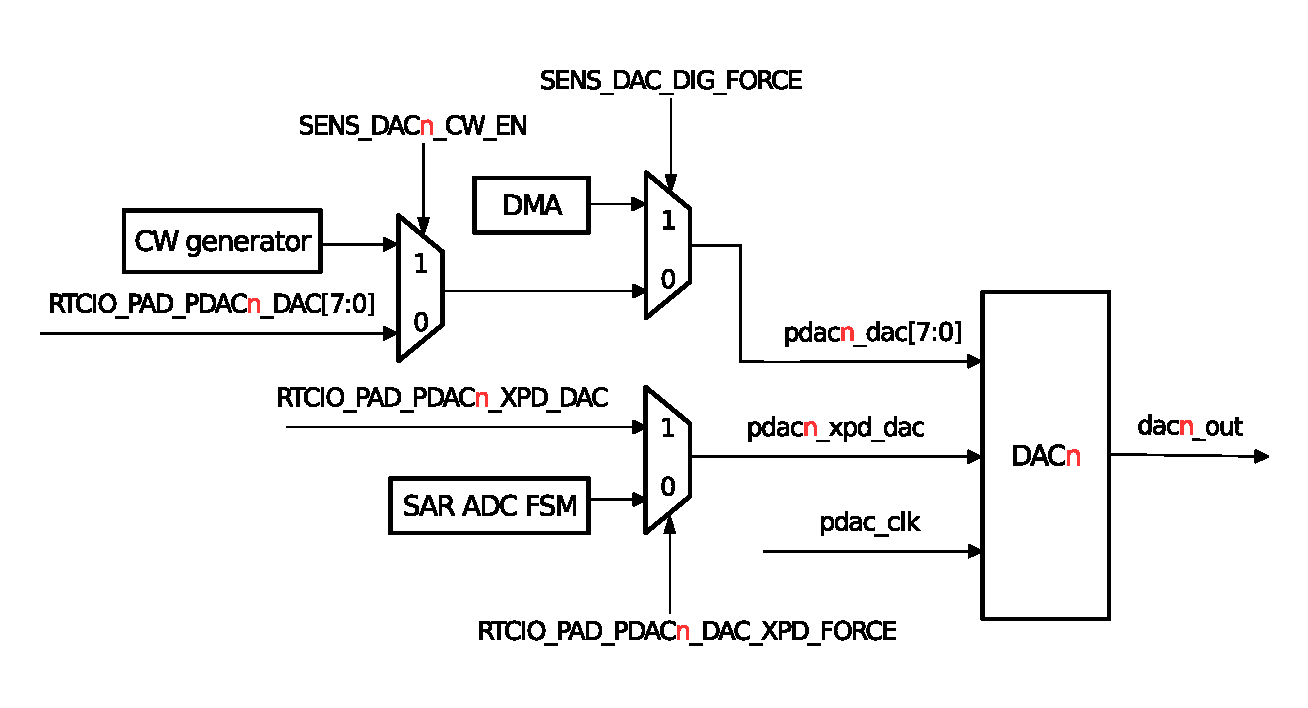
\includegraphics[width=0.8\textwidth]{./31-SENSOR/figures/dac.eps}}
    \caption{DAC 的功能概况}
    \label{figure:dac mux}
\end{figure}

\subsection{结构}\label{sec:structure}

双通道 DAC 的 2 个 8 位通道可实现独立配置，每个通道的输出模拟电压计算方式见下：
$$\mathrm{DAC\textcolor{red}{\it{n}}\_OUT = VDD3P3\_RTC \cdot PDAC\textcolor{red}{\it{n}}\_DAC / 255}$$

\begin{itemize}
    \item VDD3P3\_RTC 代表 VDD3P3\_RTC 引脚的电压(通常为 3.3V)。
    \item PDAC\textcolor{red}{\it{n}}\_DAC 拥有多个来源： \hyperref[ssec:cosine gen]{余弦波形生成器}、寄存器 \hyperref[regdesc:RTCIOPADDAC1REG]{RTCIO\_PAD\_DAC\textcolor{red}{\it{n}}\_REG}，及 DMA 。
\end{itemize}

可通过寄存器 \hyperref[regdesc:RTCIOPADDAC1REG]{RTCIO\_PAD\_PDAC\textcolor{red}{\it{n}}\_XPD\_DAC} 决定转换是否开始，软件或 SAR ADC FSM 控制转换流程本身，具体请见图 \ref{figure:dac mux}。

\subsection{余弦波形生成器}
\label{ssec:cosine gen}

余弦波形生成器可用于生成余弦波形/正弦波形，具体工作流程可见图 \ref{figure:cw gen}。

余弦波形生成器的特点包括：
\begin{itemize}
    \item 频率可调节\\
    余弦波的频率可通过寄存器 \hyperref[regdesc:SENSSARDACCTRL1REG]{SENS\_SAR\_SW\_FSTEP[15:0]} 调节：
    $$\mathrm{freq = dig\_clk\_rtc\_freq \cdot SENS\_SAR\_SW\_FSTEP / 65536}$$
    通常，dig\_clk\_rtc 的频率为 8 MHz。
    \item 振幅可调节\\
    可通过寄存器 \hyperref[regdesc:SENSSARDACCTRL2REG]{SENS\_SAR\_DAC\_SCALE\textcolor{red}{\it{n}}[1:0]} 设置波形振幅，调整为 1、1/2、1/4 或 1/8 倍。
    \item 直流偏移\\
    寄存器 \hyperref[regdesc:SENSSARREADCTRL2REG]{SENS\_SAR\_DAC\_DC\textcolor{red}{\it{n}}[7:0]} 可能引入一些直流偏移，导致结果饱和。
    \item 相位移动\\
    可通过寄存器 \hyperref[regdesc:SENSSARDACCTRL2REG]{SENS\_SAR\_DAC\_INV\textcolor{red}{\it{n}}[1:0]} 增加 0/90/180/270° 相位偏移。
\end{itemize}

\begin{figure}[!ht]
    \centering
    \fbox{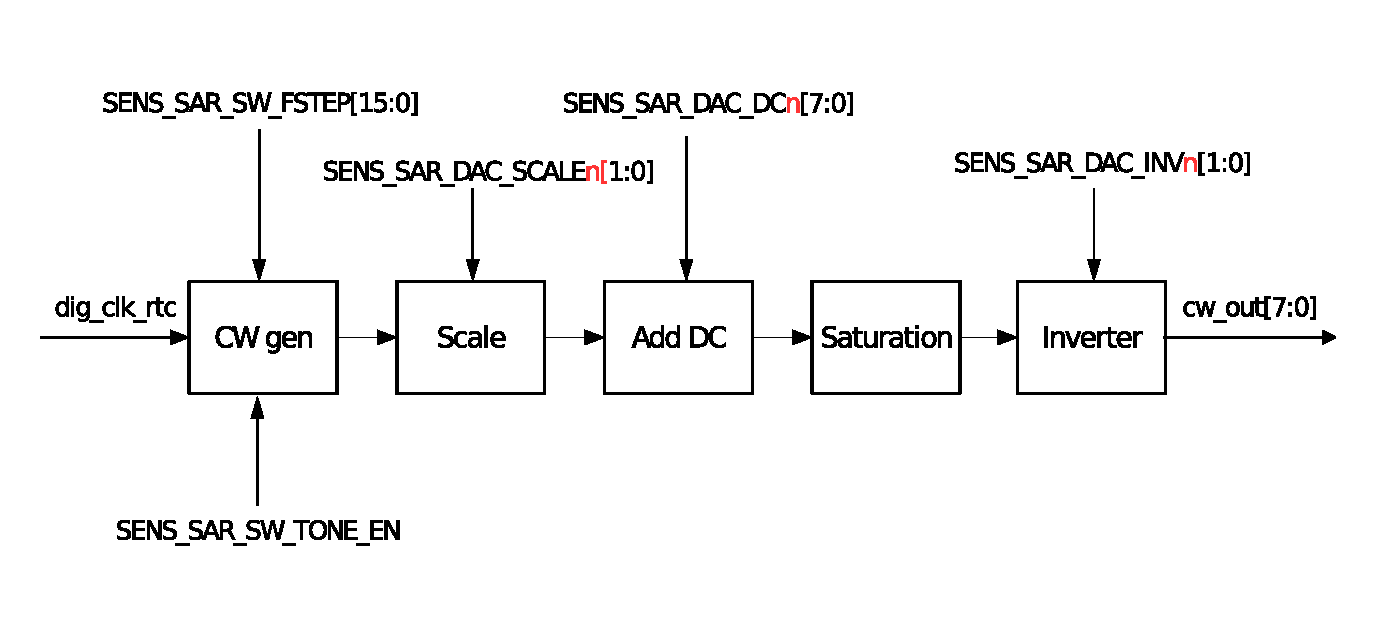
\includegraphics[width=0.8\textwidth]{./31-SENSOR/figures/dac2.eps}}
    \caption{余弦波形生成器的工作流程}
    \label{figure:cw gen}
\end{figure}

\subsection{支持 DMA}

双通道 DAC 的直接内存存取(DMA)控制器可对 2 个 DAC 通道的输出进行设置。通过配置 \hyperref[regdesc:SENSSARDACCTRL1REG]{SENS\_SAR\_DAC\_DIG\_FORCE} ，I2S\_clk 可连接至 DAC clk，I2S\_DATA\_OUT 可连接至 DAC\_DATA 实现直接内存访问。

更多信息，请见 \hyperref[paragraph: DMA]{DMA} 章节。


\hypertarget{sensor-reg-summ}{}
\section{寄存器列表}

说明：下方寄存器的分类主要以功能为主，并不反映访问内存的具体顺序。

\subsection{传感器}\label{sec:sensor-reg-summ}

请查看章节 \hyperref[glossary-access-types]{\textit{寄存器的访问类型}}，了解“访问”列缩写的含义。

\subfile{\modulefiles/sens_reg-summary_cn.tex}

\subsection{外围总线}\label{sec:apb-reg-summ}

请查看章节 \hyperref[glossary-access-types]{\textit{寄存器的访问类型}}，了解“访问”列缩写的含义。

\subfile{\modulefiles/apb_ctrl_reg-summary_cn.tex}

\subsection{RTC I/O}

有关 RTC I/O 的相关寄存器列表，请参见 \hyperref[mod:iomuxgpio]{IO\_MUX 和 GPIO 交换矩阵}章节中\hyperref[section:4.12]{寄存器列表}的内容。
\newpage

\section{寄存器}
\label{section:registers}

\subsection{传感器}

本小节括号中的地址均为相对于 (RTC 基地址 + 0x0800) 的地址偏移量（相对地址）。RTC 基地址见章节 \ref{mod:sysmem} \textit{\nameref{mod:sysmem}} 中的表 \ref{table:Peripheral_Address_Mapping} \textit{外设地址映射}。寄存器绝对地址见章节 \ref{sec:sensor-reg-summ} \textit{\nameref{sec:sensor-reg-summ}}。

关于保留 (reserved) 域的处理，请查看章节 \hyperref[programming-reserved-field]{\textit{如何配置寄存器的保留域}}。

\subfile{\modulefiles/sens_reg_cn.tex}

\subsection{高级外围总线}

本小节括号中的地址均为相对于 0x6000\_2600 的地址偏移量（经 AHB 总线访问）。寄存器绝对地址见章节 \ref{sec:apb-reg-summ} \textit{\nameref{sec:apb-reg-summ}}。

关于保留 (reserved) 域的处理，请查看章节 \hyperref[programming-reserved-field]{\textit{如何配置寄存器的保留域}}。

\subfile{\modulefiles/apb_ctrl_reg_cn.tex}

\subsection{RTC I/O}

有关 RTC I/O 的相关寄存器，请参见 \hyperref[mod:iomuxgpio]{IO\_MUX 和 GPIO 交换矩阵}章节中\hyperref[section:4.13]{寄存器}的内容。

\end{document}
